\chapter{案例分析}
\section{案例實驗設計}
\indent
本論文將以自行設計之Microsoft網頁相關測試專案作為實驗腳本,其中含有十一個測試套件、七個測試資源,是屬於規模較小的測試專案,此實驗將以團隊最常使用的Visual Studio Code搜尋取代工具及擴充後之RF Refactoring進行重構,其重構方法為抽取測試腳本之重複步驟成為新關鍵字及移動關鍵字宣告兩種。

\indent
本論文將參考陳昱仁論文\cite{Experiment_Settings}實驗分析中的實驗設計方法,邀請國立台北科技大學軟體系統實驗室之測試團隊成員,協助使用兩種工具進行重構並比較其時間差異,以此確認擴充後之重構工具對於團隊是否有實質之幫助。在開始測驗之前,將會帶領每位測試人員了解該測試專案所要測試的網頁內容,使其對測試專案先有一定的了解。因為現有環境上的限制,只能請測試人員務必於只有一人的環境中進行測驗,並且確保其餘可能影響實驗準確性之外在因素皆不存在,例如:手機、通訊軟體等等,最後為每位測試人員解釋各個案例狀況後即開始進行測驗。

\section{案例一:抽取測試腳本中的重複步驟成為新關鍵字並引入所需測試資源}\label{s5.1}
\indent
程式碼\ref{l5.1}為測試專案的測試套件之一,其含有一個測試案例,用來測試前往Windows安全性頁面之功能,並且測試其功能正常後,於報表中印出歡迎相關之訊息。程式碼\ref{l5.2}同為測試專案中的測試套件,同樣含有一個測試案例,用來測試前往Windows10功能頁面之功能,於功能驗證完成後,在報表中印出歡迎相關之訊息。

\indent
比對程式碼\ref{l5.1}(18-20行)及程式碼\ref{l5.2}(18-20行)可以發現,其在於功能驗證後都會印出歡迎相關之訊息,因此可以將它們認定為重複步驟並進行重構。此測試專案中共有四個測試案例都擁有重複之步驟,需要將其抽取成新關鍵字並取代後,引入其所需之測試資源,因此本論文邀請五位測試團隊成員依照下列小節之方式,進行相對應之重構,並於後續比較其使用差異。

\begin{lstlisting}[caption=前往Windows安全性頁面之測試套件, label={l5.1}]
9   *** Variables ***
10  @{welcomeTaipei} =    Welcome    To    Taipei
11  
12  *** Test Cases ***
13  Go To "Windows Security" Page And Log Welcome Text
14      Go To Windows Page
15      Open Windows 10 Menu
16      Go To "Windows Security" Page
17      "Windows Security" Page Should Be Visible
18      FOR    ${var}    IN    @{welcomeTaipei}
19          Log Double Text    ${var}
20      END
21      [Teardown]    Close Browser
\end{lstlisting}

\begin{lstlisting}[caption=前往Windows10功能頁面之測試套件, label={l5.2}]
9   *** Variables ***
10  @{welcomeTainan} =    Welcome    To    Tainan
11
12  *** Test Cases ***
13  Go To "Windows 10 features" Page And Log Welcome Text
14      Go To Windows Page
15      Open Windows 10 Menu
16      Go To "Windows 10 features" Page
17      "Windows 10 features" Page Should Be Visible
18      FOR    ${var}    IN    @{welcomeTainan}
19          Log Double Text    ${var}
20      END
21      [Teardown]    Close Browser
\end{lstlisting}
\newpage

\subsection{使用Visual Studio Code搜尋取代工具}\label{s5.1.1}
\indent
首先利用Visual Studio Code(VSCode)將重複步驟複製至目標測試資源中,以其做了什麼為新關鍵字之名稱,且將未宣告於步驟內之變數作為新關鍵字之參數,藉此創立新關鍵字,結果如程式碼\ref{l5.3}。後續於搜尋工具中,以重複步驟之關鍵字為搜尋目標,搜尋結果如圖\ref{f5.1}所示,其中一個搜尋結果為關鍵字之宣告,非所需之重複步驟故不取代,其餘四個結果分別與重複步驟之參數數量、關鍵字順序及關鍵字名稱相同,因此以新關鍵字進行取代。

\indent
後續於已進行重複步驟取代之測試套件,檢查其是否有引入新關鍵字所需之測試資源,為未引入者進行引入之動作。

\begin{lstlisting}[caption=新關鍵字架構, label={l5.3}]
Log Welcome Text
    [Arguments]    ${welcomeTexts}
    FOR    ${var}    IN    @{welcomeTexts}
        Log Double Text    ${var}
    END
\end{lstlisting}

\begin{figure}[H]
   \centering
   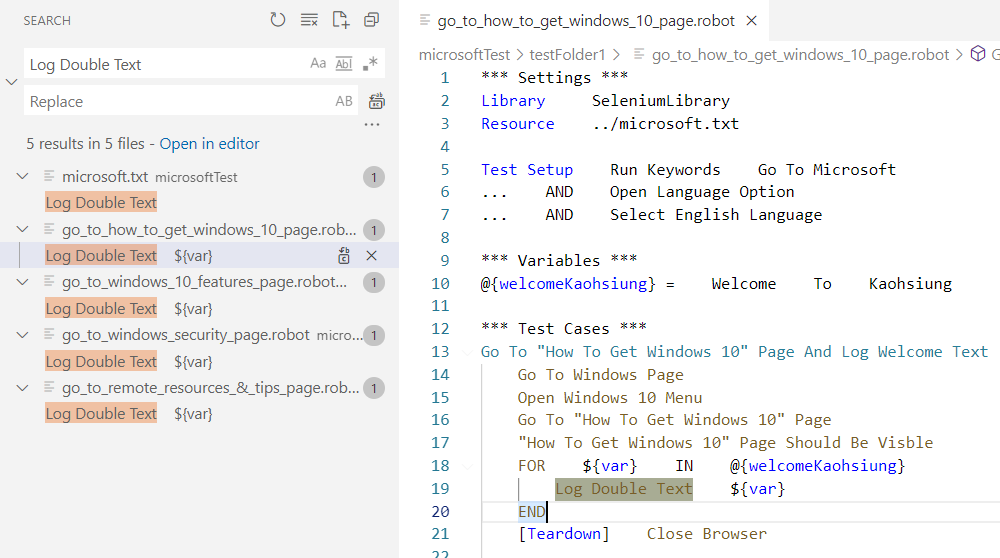
\includegraphics[width=0.9\textwidth]{picture/ch5/vscode_search_in_case1.PNG}
   \caption{重複步驟搜尋結果}
   \label{f5.1}
\end{figure}

%\begin{figure}[H]
%	\centering
%	\begin{minipage}[b]{0.43\textwidth}
%		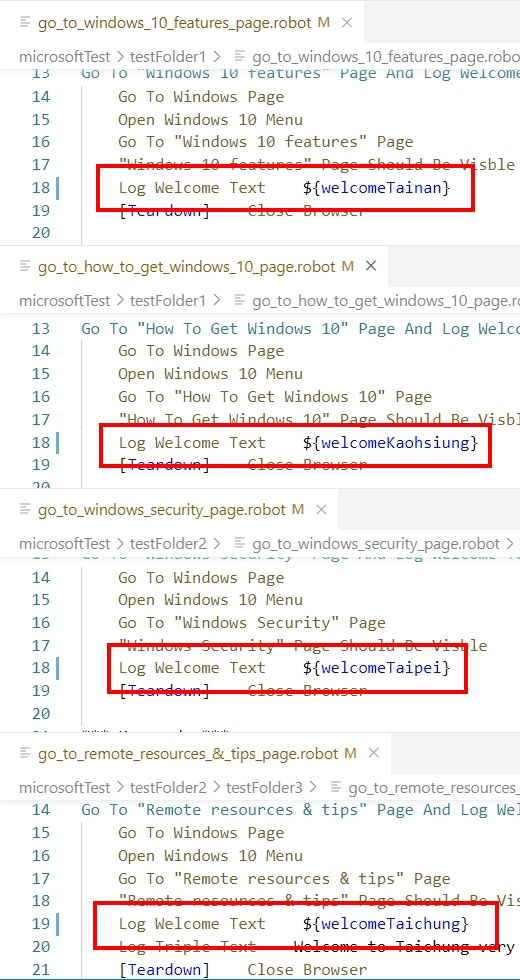
\includegraphics[width=1.05\textwidth]{picture/ch5/After_replace_with_new_keyword_in_case1.png}
%		\caption{關鍵字取代重複步驟後結果}
%		\label{f5.2}
%	\end{minipage}
%	\begin{minipage}[b]{0.53\textwidth}
%		\centering
%		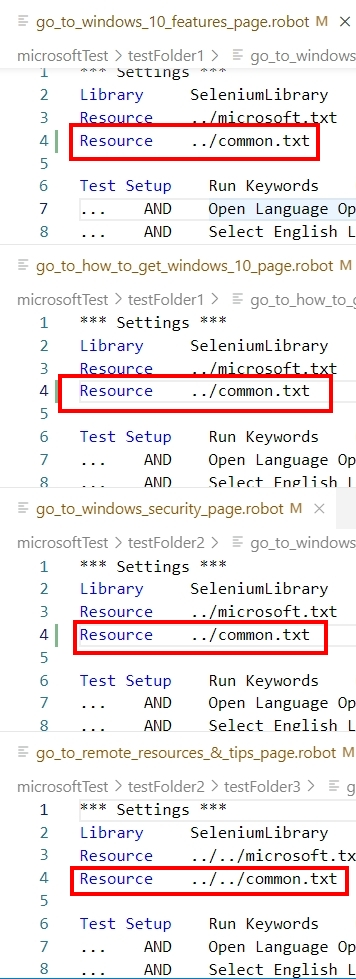
\includegraphics[width=0.85\textwidth]{picture/ch5/Import_resource_in_case1.png}
%		\caption{引入新關鍵字所需之測試資源結果}
%		\label{f5.3}
%	\end{minipage}
%\end{figure}

\subsection{使用擴充後之RF Refactoring}\label{s5.1.2}
\indent
後續使用擴充後之RF Refactoring的Wrap Steps As A New Keyword功能重構\ref{s5.1}節所提及之重複步驟,選取其中一個測試套件中的重複步驟,其將會自動把未宣告於步驟中的變數加入新關鍵字的參數,如圖\ref{f5.4}所示,於此視窗可以同時決定新關鍵字之名稱,並且創立新關鍵字於圖\ref{f5.5}視圖中所選擇之檔案。根據專案下所檢查出含有重複步驟的測試套件,其可在圖\ref{f5.6}之視圖中選擇要以新關鍵字取代之重複步驟,並且為每個要使用的新關鍵字決定其參數實際值,以此完成重複步驟之取代,最後RF Refactoring將自動引入新關鍵字所需之測試資源。

\begin{figure}[H]
    \centering
    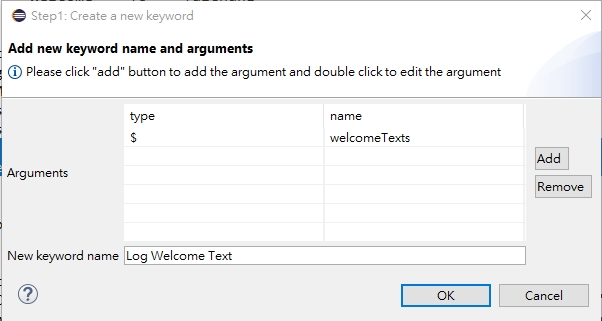
\includegraphics[width=0.7\textwidth]{picture/ch5/Eclipse_create_keyword_in_case1.png}
    \caption{創立新關鍵字視窗結果}
    \label{f5.4}
\end{figure}

\begin{figure}[H]
    \centering
    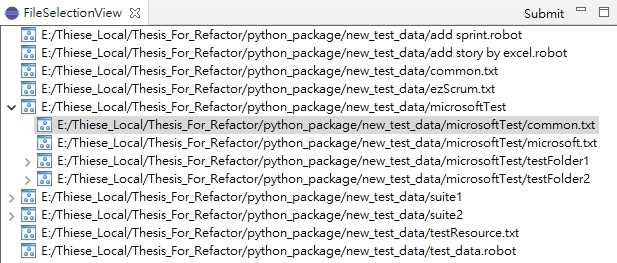
\includegraphics[width=0.7\textwidth]{picture/ch5/Eclipse_choose_file_to_create_keyword_in_case1.png}
    \caption{專案下檔案顯示視圖結果}
    \label{f5.5}
\end{figure}

\begin{figure}[H]
    \centering
    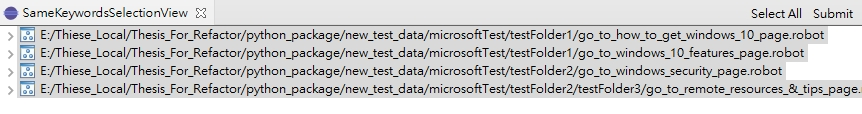
\includegraphics[width=0.7\textwidth]{picture/ch5/Eclipse_choose_duplicate_steps_in_case1.png}
    \caption{搜尋重複步驟結果之視圖}
    \label{f5.6}
\end{figure}

%\begin{figure}[H]
%	\centering
%	\begin{minipage}[b]{0.43\textwidth}
%		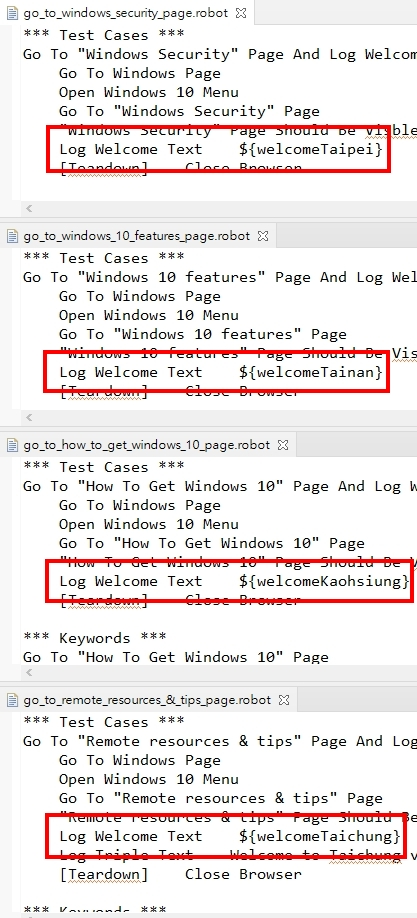
\includegraphics[width=1.05\textwidth]{picture/ch5/Eclipse_replace_result_in_case1.png}
%		\caption{關鍵字取代重複步驟後結果}
%		\label{f5.7}
%	\end{minipage}
%	\begin{minipage}[b]{0.53\textwidth}
%		\centering
%		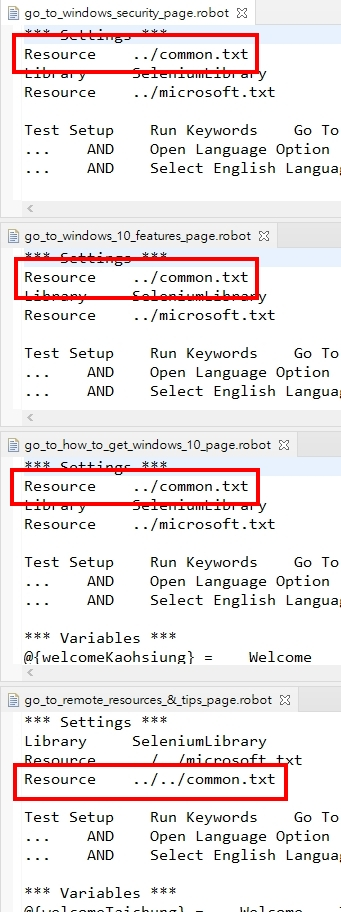
\includegraphics[width=0.85\textwidth]{picture/ch5/Eclipse_Import_resource_result_in_case1.png}
%		\caption{引入新關鍵字所需之測試資源結果}
%		\label{f5.8}
%	\end{minipage}
%\end{figure}

\subsection{重構工具使用之比較}

\begin{table}[H]
    \begin{center}
    \caption{使用兩種工具包裹重複步驟成為新關鍵字並引入所需測試資源之比較}\label{t5.1}
        \begin{tabular}{|c|c|c|}\hline
                             & 使用VSCode重構花費之時間    & 使用擴充後之RF Refactoring重構花費之時間    \\\hline
        測試人員1           & 06m02s          & 03m24s    \\\hline
        測試人員2           & 05m12s          & 04m20s    \\\hline
        測試人員3           & 07m31s          & 04m20s    \\\hline
        測試人員4           & 06m20s          & 04m59s    \\\hline
        測試人員5           & 06m29s          & 06m07s    \\\hline
\textbf{平均時間}           & \textbf{06m18s} & \textbf{04m38s}    \\\hline
        \end{tabular}
    \end{center}
\end{table}
\indent
表\ref{t5.1}為紀錄團隊測試人員使用兩種不同工具進行此重構之比較,從表中可見每一位測試人員根據經驗之不同,使用VSCode進行重構所花費之時間也略微不同,平均大約花費了6分18秒,並且重構過程中,測試人員有三位不小心忽視了新關鍵字所需之測試資源,導致測試失敗;而使用擴充後之RF Refactoring重構時,平均大約花費了4分38秒,並且未有測試資源沒被引入之狀況發生。由此比較可發現,使用擴充後之RF Refactoring進行此重構時,因為不需要手動搜尋重複步驟以及檢查所需之測試資源是否引入,能夠花費較少的時間,其大約減少了26.4\%的時間,並且較不容易發生錯誤。

\section{案例二:移動測試資源中的關鍵字宣告並引入所需測試資源}\label{s5.2}
\indent
程式碼\ref{l5.4}為測試專案的測試套件之一,其中第5行之Go To Microsoft關鍵字於其他測試套件剛好也需要使用,因此必須將其之宣告移動至共用之測試資源,以便其他測試套件使用。在移動到目標測試資源後,必須檢查原先已使用此關鍵字之四個測試套件是否都有引入其所需之測試資源,避免發生未宣告關鍵字之錯誤。

\indent
根據此案例之重構,本論文邀請與\ref{s5.1}節相同之五位測試團隊成員使用下列小節之方式,進行相對應之重構,最後比較其使用差異。

\begin{lstlisting}[caption=前往如何取得Windows10頁面之測試套件, label={l5.4}]
1   *** Settings ***
2   Library     SeleniumLibrary
3   Resource    ../microsoft.txt
4
5   Test Setup    Run Keywords    Go To Microsoft
6   ...    AND    Open Language Option
7   ...    AND    Select English Language

8   *** Variables ***
9   @{welcomeKaohsiung} =    Welcome    To    Kaohsiung
10
11  *** Test Cases ***
12  Go To "How To Get Windows 10" Page And Log Welcome Text
13      Go To Windows Page
14      Open Windows 10 Menu
15      Go To "How To Get Windows 10" Page
16      "How To Get Windows 10" Page Should Be Visible
17      Log Welcome Text    ${welcomeKaohsiung}
18      [Teardown]    Close Browser
\end{lstlisting}

\subsection{使用Visual Studio Code搜尋取代工具}
\indent
首先利用VSCode將需要移動之關鍵字宣告於其所在檔案中移除,並在共用測試資源上完整複製遭移除之關鍵字宣告,後續於搜尋工具之視窗,以被移動之關鍵字名稱進行搜尋,搜尋結果如圖\ref{f5.9}所示,其中一個搜尋結果為關鍵字之宣告的,故不需檢查,其餘結果皆為原先已使用此關鍵字之測試套件。接著於每個測試套件中搜尋是否有引入共用之測試資源,如否則為其引入以避免測試錯誤。

\begin{figure}[H]
    \centering
    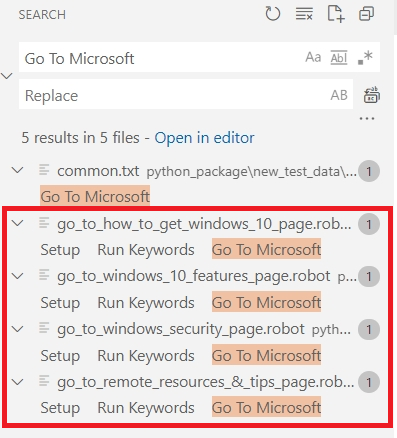
\includegraphics[width=0.35\textwidth]{picture/ch5/Search_using_keyword_in_case2.png}
    \caption{搜尋使用被移動關鍵字之測試套件結果}
    \label{f5.9}
\end{figure}

%\begin{figure}[H]
%	\centering
%	\begin{minipage}[b]{0.5\textwidth}
%		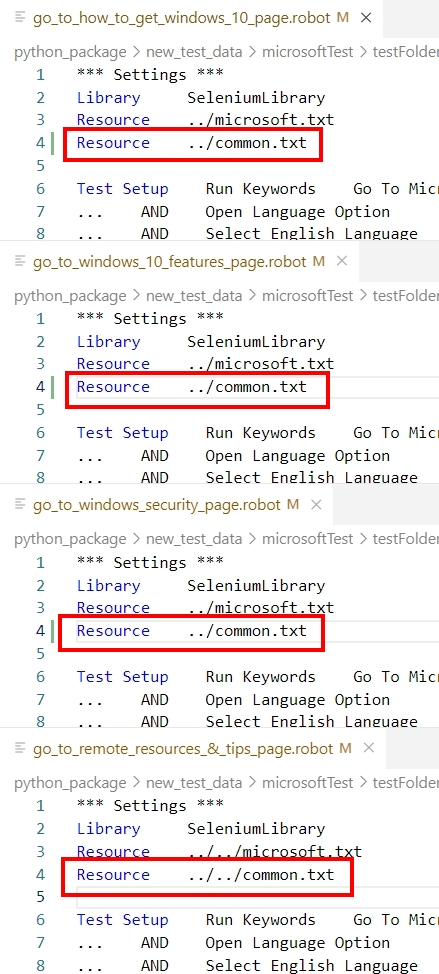
\includegraphics[width=0.8\textwidth]{picture/ch5/Import_resource_in_case2.png}
%		\caption{引入關鍵字所需之測試資源結果}
%		\label{f5.10}
%	\end{minipage}
%	\begin{minipage}[b]{0.48\textwidth}
%		\centering
%		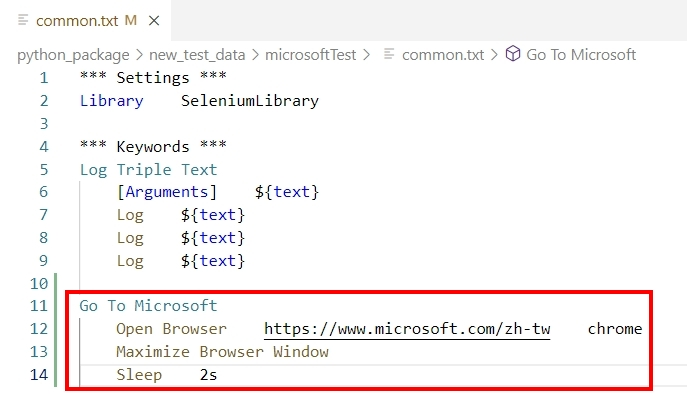
\includegraphics[width=1.2\textwidth]{picture/ch5/Move_keyword_result_in_case2.png}
%		\caption{關鍵字宣告移動之結果}
%		\label{f5.11}
%	\end{minipage}
%\end{figure}

\subsection{使用擴充後之RF Refactoring}
\indent
接著使用擴充後之RF Refactoring的Move Keyword Defined To Another File功能重構\ref{s5.2}節所提及的需移動之關鍵字宣告,選取其關鍵字名稱後,即可將關鍵字宣告移動至圖\ref{f5.12}視圖中所選取之目標檔案,後續RF Refactoring將自動為原先已使用此關鍵字之測試套件引入所需測試資源。

\begin{figure}[H]
    \centering
    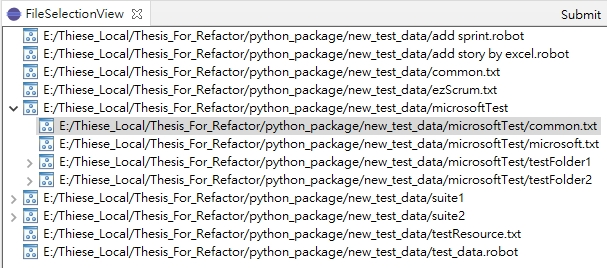
\includegraphics[width=0.7\textwidth]{picture/ch5/Eclipse_choose_file_in_case2.png}
    \caption{專案下全部測試檔案之視圖}
    \label{f5.12}
\end{figure}

%\begin{figure}[H]
%	\centering
%	\begin{minipage}[b]{0.48\textwidth}
%		\centering
%		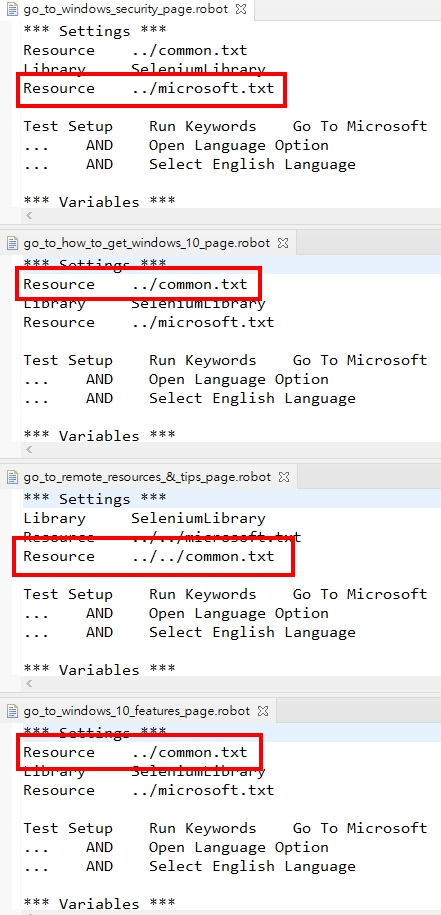
\includegraphics[width=0.9\textwidth]{picture/ch5/Eclipse_import_resource_in_case2.png}
%		\caption{引入關鍵字所需測試資源之結果}
%		\label{f5.13}
%	\end{minipage}
%	\begin{minipage}[b]{0.5\textwidth}
%		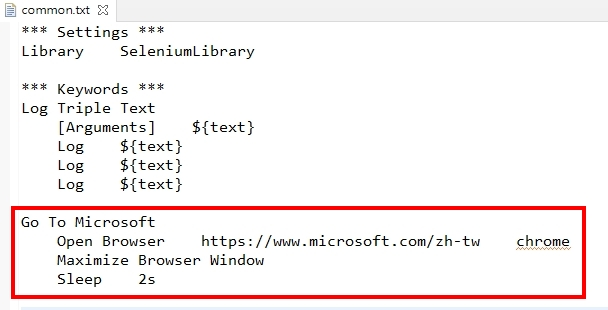
\includegraphics[width=1.2\textwidth]{picture/ch5/Eclipse_move_keyword_result_in_case2.png}
%		\caption{關鍵字宣告移動之結果}
%		\label{f5.14}
%	\end{minipage}
%\end{figure}

\subsection{重構工具使用之比較}

\begin{table}[H]
    \begin{center}
    \caption{使用兩種工具移動關鍵字宣告並引入所需測試資源之比較}\label{t5.2}
        \begin{tabular}{|c|c|c|}\hline
                & 使用VSCode重構花費之時間 & 使用擴充後之RF Refactoring重構花費之時間    \\\hline
        測試人員1      & 01m14s             & 00m26s    \\\hline
        測試人員2      & 01m35s             & 00m18s    \\\hline
        測試人員3      & 01m17s             & 00m22s    \\\hline
        測試人員4      & 01m00s             & 00m26s    \\\hline
        測試人員5      & 02m02s             & 00m41s    \\\hline
\textbf{平均時間}      & \textbf{01m25s}    & \textbf{00m26s}    \\\hline
        \end{tabular}
    \end{center}
\end{table}
\indent
表\ref{t5.2}為紀錄團隊測試人員使用兩種不同工具進行此重構之比較,從表中可發現,使用VSCode進行重構時,平均花費了1分25秒,且有兩位測試人員對於部分測試套件有錯誤引入關鍵字所需測試資源之相對路徑,導致測試錯誤;而使用擴充後之RF Refactoring重構時,平均花費了26秒,且引入所需測試資源之路徑皆為正確。從此比較可發現,使用擴充後之RF Refactoring進行此重構時,因為不需要自我檢查測試套件是否都有引入所需之測試資源,能夠花費較少的時間,其大約減少了69.4\%的時間,並且較不容易因人為檢查缺漏而發生錯誤。